\chapter{Les différentes techniques de cryptographie}

\section{Les chiffres de substitution}
Cette méthode consiste à simplement remplacer une lettre, un ensemble
de lettres (un \emph{polygramme}), un mot, ...  par une autre lettre,
polygramme, ou bien par un nombre ou un signe.

On peut distinguer plusieurs sortes de substitutions : 
\begin{itemize}
  \renewcommand{\makelabel}[1]{\sffamily\textbf{#1}}
  \item[Les substitutions monoalphabétiques ou simples] : 
    chaque lettre est remplacée par une autre lettre tout au long du message~; 
  \item[Les substitutions polyalphabétiques] :
    c'est en fait une combinaison de substitutions simples~;
  \item[Les substitutions polygrammiques]: 
    à la place de substituer des lettres comme le fait la substitution
    monoalphabétique, on substitue des groupes de lettres~;
  \item[Les substitutions homophoniques] : 
    chaque lettre peut être remplacée par plusieurs valeurs, choisies
    aléatoirement.
\end{itemize}

\note{Dans ce chapitre, nous ferons abstraction des caractères
  spéciaux, comme les lettres avec accents, des signes de
  ponctuations, ou autre caractères. Nous remplacerons ceux-ci par une
  espace si besoin est.}

\subsection{Les substitutions monoalphabétiques}
Ce type de substitution consiste simplement à remplacer chaque lettre
de l'alphabet par une autre lettre.

\subsubsection{Par simple décalage}
On peut par exemple, comme le fait le chiffre de
César\footref{syst:chiffrecesar}, décaler les lettres de l'alphabet d'une
clé $k$. \\

 Si nous considérons l'alphabet comme un ensemble cyclique où 
chaque lettre correspondrait à un chiffre (une fois arrivé à $Z$ ($= 25$), on 
repart de $A$ ($= 0$) $\rightarrow 25 + 1 = 0$), on peut facilement définir 
ce système de chiffrement :  \\

\definition{$e_k(c) = (c + k)~ mod~ 26$\\
  où $c$ est le caractère à chiffrer.}

Nous utilisons l'opérateur \emph{modulo}, qui nous donne le reste de
la division entière de deux entiers ($5~ mod~ 2 = 1$), ce qui nous
permet de rester dans un ensemble cyclique. \\

\paragraph{Exemple: le rot13\label{syst:rot13}}
Une application du chiffre de César est, par exemple, le \emph{ROT13},
qui est simplement un chiffre de César pour lequel la clé $k$ a une
valeur de $13$.\\

L'interêt du ROT13 réside dans le fait qu'il suffit d'appliquer deux
fois la méthode de chiffrement pour retrouver le texte en clair
($e_{13}(e_{13}(M)) = M$), ainsi, il n'y a qu'une et une seule fonction utilisée
pour le chiffrement et le déchiffrement (donc $e_{13}(x) =
d_{13}(x)$). \\

De ce fait, ROT13 n'est pas du tout pratique pour cacher des
informations, mais est parfois utilisé sur internet, dans les forums,
afin d'empêcher la lecture involontaire d'un texte (qui pourrait
dévoiler une information sur un film par exemple, et gâcherait le
plaisir au gens n'ayant pas vu le film, c'est ce qu'on appelle un 
\emph{spoiler}) 

\subsubsection{Par remplacement}
Outre le fait de décaler les lettres, on peut aussi remplacer chaque
lettre de l'alphabet par une autre lettre. Pour chiffrer, on peut alors
s'aider d'une table de substitution, comme sur la figure
\ref{fig:SubstitutionSimple}.

 \begin{figure}[h]
   \begin{center}
    \begin{tabular}{|c|c|c|c|c|c|c|c|c|c|c|c|c|c|c|c|c|c|c|c}
      \hline
      A & B & C & D & E & F & G & H & I & J & K & L & M & N & O & P &
      Q & R & S & T \\
      \hline
      A & Z & E & R & T & Y & U & I & O & P & Q & S & D & F & G & H &
      J & K & L & M \\
      \hline
    \end{tabular}
  \end{center}
  \begin{flushright}
    \begin{tabular}{c|c|c|c|c|c|}
      \hline
      U & V & W & X & Y & Z \\
      \hline
      W & X & C & V & B & N \\
      \hline
    \end{tabular}
  \end{flushright}
  \caption{Exemple simple de table de substitution}
  \label{fig:SubstitutionSimple}
\end{figure}

Dans cette table de substitution, on peut placer les lettre
aléatoirement, selon une règle, ou en utilisant une clé (qu'on notera
en début de table, et nous recopierons les caractères non utilisés par
après, voir la figure \ref{fig:SubstitutionCle}).

\begin{figure}[h]
  \begin{center}
    \begin{tabular}{|c|c|c|c|c|c|c|c|c|c|c|c|c|c|c|c|c|c|c|c}
      \hline
      A & B & C & D & E & F & G & H & I & J & K & L & M & N & O & P &
      Q & R & S & T \\
      \hline
      C & R & Y & P & T & O & A & B & D & E & F & G & H & I & J & K &
      L & M & N  & Q  \\
      \hline
    \end{tabular}
  \end{center}
  \begin{flushright}
    \begin{tabular}{c|c|c|c|c|c|}
      \hline
      U & V & W & X & Y & Z  \\
      \hline
      S & U & V & W & X & Z \\
      \hline
    \end{tabular}
  \end{flushright}
  \caption{Exemple de table de substitution avec comme clé ``crypto''}
  \label{fig:SubstitutionCle}
\end{figure}

Il existe de nombreuses méthodes dans le même genre pour remplacer
simplement une lettre par une autre, voyons en une de plus près :
\emph{le carré de Polybe.}\\

\paragraph{Exemple: le carré de Polybe\label{syst:CarrePolybe}}
Polybe est un historien grec (210 av. J.-C., 126 av. J.-C.), qui
explique vers 150 av. J.-C. une méthode de chiffrement par
substitution assez simple et intéressante.\\

Cette méthode consiste à placer les lettres de l'alphabet dans un
carré de 25 cases (il faut donc retirer une lettre, le W pour le
français, qui sera remplacé par V dans le message). La lettre chiffrée
sera remplacée par un nombre formé par le numéro de la colonne et de
la ligne de la lettre.\\

Nous pouvons représenter ce carré par une matrice de taille $5\times 5$
(voir la figure \ref{fig:Polybe}). Nous pouvons, analogiquement à la
figure \ref{fig:SubstitutionCle}, utiliser une clé pour le carré de
Polybe. \\

Le carré de Polybe est assez intéressant car il convertit les lettres
en chiffres et réduit le nombre de symbole utilisés dans le message
chiffrés (9 chiffres plutôt que 26 lettres). \\

\begin{figure}[h]
  $
  \left(
    \begin{array}{ccccc}
      A & B & C & D & E \\
      F & G & H & I & J \\
      K & L & M & N & O \\
      P & Q & R & S & T \\
      U & V & X & Y & Z
    \end{array}
  \right)
  $
  \hfill
  $
  \left(
    \begin{array}{ccccc}
      C & R & Y & P & T \\
      O & A & B & D & E \\
      F & G & H & I & J \\
      K & L & M & N & Q \\
      S & U & V & X & Z
    \end{array}
  \right)
  $
  \hfill
  $
  \left(
    \begin{array}{ccccc}
      a_{11} & a_{12} & a_{13} & a_{14} & a_{15}  \\
      a_{21} & a_{22} & a_{23} & a_{24} & a_{25}  \\
      a_{31} & a_{32} & a_{33} & a_{34} & a_{35}  \\
      a_{41} & a_{42} & a_{43} & a_{44} & a_{45}  \\
      a_{51} & a_{52} & a_{53} & a_{54} & a_{55}
    \end{array}
  \right)
  $
  \caption{Le carré de Polybe sous forme de matrice, la seconde
    matrice ayant comme clé « crypto », et la troisième représentant
    les nombres par lesquels seront remplacés les caractères dans le
    message chiffré.}
  \label{fig:Polybe}
\end{figure}

Polybe imaginait un moyen de communiquer les messages via des torches
: le nombre de torches placée à gauche correspondrait au numéro de la
ligne, et le nombre de torches à droit au numéro de la colonne. \\

Le carré de Polybe était utilisé par les nihilistes russes entre le
XIX\ieme~ et le XX\ieme~ siècle (des « terroristes » dont le but était de
% TODO: eme
tuer le tsar pour reconstruire une société sur de nouvelles
bases). Lorsqu'ils étaient attrapés et enfermés en prison, ils
communiquaient via le carré de Polybe, en donnant des coups sur les
murs. \\ %TODO: mieux expliquer

\begin{figure}[h]
  \begin{center}
    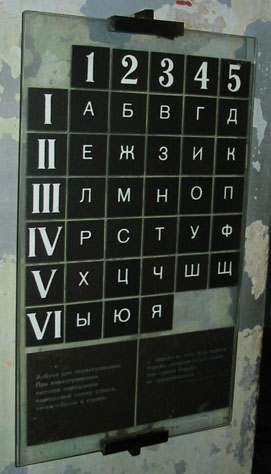
\includegraphics[scale=1.5]{eps/Nihilistes}
  \end{center}
  \caption{Version du carré de Polybe utilisée par les nihilistes
    russes}
  \label{fig:Nihilistes}
\end{figure}

\subsection{Les substitutions polyalphabétiques\label{SubstitutionPolyalphabetique}}
Les substitutions polyalphabétiques sont une combinaison de plusieurs
tables de substitutions simples, où l'on change de table à chaque
lettre, ce qui rend le message chiffré beacoup plus dur à casser sans
le code (nous verrons ceci en détail dans le chapitre
\ref{Cryptanalyse}, page \pageref{Cryptanalyse} sur la cryptanalyse)

Une des substitutions polyalphabétiques les plus connues est le
\emph{Chiffre de Vigenère}.

\paragraph{Exemple : Le chiffre de Vigenère\label{syst:ChiffreVigenere}}
Au XIX\ieme~ siècle, Vigenère « invente » une nouvelle méthode de
chiffrement en s'inspirant fortement des travaux de l'abbé allemand
Jean Trithème du XVI\ieme~ siècle. Blaise de Vigenère a néanmoins
modifié légèrement la méthode de Trithème en rendant l'utilisation de
clé de chiffrement possible.\\

La technique de Jean Trithème est d'utiliser ce qu'il décrit comme une
\emph{tabula recta}
\ref{fig:TabulaRecta}) qui est composée de 24 rangées de 24
lettres chacune. On retire donc deux lettres, le J et le V, qui seront
respectivement remplacées par le I et le W. Le W est placé après le
Z.\\
Chaque rangée correspond à un chiffre de César\footref{syst:chiffrecesar},
avec à chaque fois un décalage augmenté d'une unité. \\

Par exemple, pour chiffrer le mot « cryptographie » avec la table se
trouvant à la figure \ref{fig:TabulaRecta}~: 
\begin{itemize}
  \item la lettre C est chiffrée sur la première ligne, et reste
    donc C~;
  \item la lettre R est chiffrée sur la 2\ieme~ ligne, et devient
    S. Pour cela, trouvez la colonne de R dans la première rangée, et
    descendez d'une ligne~;
  \item La lettre Y devient W (même colonne, deux rangées plus bas)~;
  \item Et ainsi de suite ~\dots~;
  \item « cryptographie » sera donc chiffré en « csasztnwiwsur ».
\end{itemize}

\begin{figure}[h]
  \begin{center}
    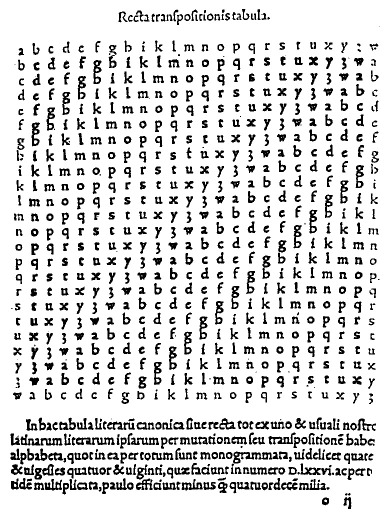
\includegraphics[scale=0.3]{eps/TabulaRecta}
  \end{center}
  \caption{La \emph{tabula recta} de Jean Trithème}
  \label{fig:TabulaRecta}
\end{figure}

Vigenère reprends donc cette méthode pour légèrement la modifier (y
ajouter l'utilisation d'une clé en fait), et la publie dans son livre
\emph{Traicté des chiffres, ou secretes
  manieres d'escrire} en 1586. \\

Comme pour la méthode de Trithème, on utilise une table, composée
cette fois ci des 26 chiffres de César possibles, comme sur la figure
\ref{fig:VigenereTableau} (Trithème en décrivait 24 dans son livre,
mais on pourrait très bien aussi en utiliser 26). \\

Expliquons cette méthode au travers d'un exemple : chiffrons « chiffre
de vigenere » avec comme mot cle « crypto ».
\begin{itemize}
  \item Tout d'abord, chaque lettre du message est associée à une
    lettre de la clé, de la façon suivante : \\
    \begin{tabular}{c@{}c@{}c@{}c@{}c@{}c@{}cc@{}cc@{}c@{}c@{}c@{}c@{}c@{}c@{}c}
      c & h & i & f & f & r & e &
      d & e &
      v & i & g & e & n & e & r & e \\

      c & r & y & p & t & o & c & 
      r & y & 
      p & t & o & c & r & y & p & t \\
    \end{tabular}\\
    La clé est donc répétée successivement~;
  \item Ensuite, chaque lettre du message clair est décalée du nombre
    de rang correspondant à la lettre de la clé qui lui est
    associée. Ainsi, pour la première lettre, C, on la décale de 2
    rangs (la lettre C lui étant associée, et la place de cette lettre
    dans l'alphabet en partant de 0 est 2). Pour s'aider, on peut
    utiliser la table du chiffre de Vigenère (voir la figure
    \ref{fig:VigenereTableau}). \\
    Ainsi, C est chiffré en E.
  \item Et on continue ainsi de suite, H est chiffré en Y, \dots
  \item « chiffre de vigenere » sera donc chiffré en « eyguyfg uc
    kbugecgx »
\end{itemize}

\begin{figure}[h]
  \begin{center}
    \begin{tabular}{c|c@{}c@{}c@{}c@{}c@{}c@{}c@{}c@{}c@{}c@{}c@{}c@{}c@{}c@{}c@{}c@{}c@{}c@{}c@{}c@{}c@{}c@{}c@{}c@{}c@{}c}
        & A & B & C & D & E & F & G & H & I & J & K & L & M & N & O & P & Q & R & S & T & U & V & W & X & Y & Z \\
      \hline
      A & A & B & C & D & E & F & G & H & I & J & K & L & M & N & O & P & Q & R & S & T & U & V & W & X & Y & Z \\
      B & B & C & D & E & F & G & H & I & J & K & L & M & N & O & P & Q & R & S & T & U & V & W & X & Y & Z & A \\
      C & C & D & E & F & G & H & I & J & K & L & M & N & O & P & Q & R & S & T & U & V & W & X & Y & Z & A & B \\
      D & D & E & F & G & H & I & J & K & L & M & N & O & P & Q & R & S & T & U & V & W & X & Y & Z & A & B & C \\
      E & E & F & G & H & I & J & K & L & M & N & O & P & Q & R & S & T & U & V & W & X & Y & Z & A & B & C & D \\
      G & G & H & I & J & K & L & M & N & O & P & Q & R & S & T & U & V & W & X & Y & Z & A & B & C & D & E & F \\
      H & H & I & J & K & L & M & N & O & P & Q & R & S & T & U & V & W & X & Y & Z & A & B & C & D & E & F & G \\
      I & I & J & K & L & M & N & O & P & Q & R & S & T & U & V & W & X & Y & Z & A & B & C & D & E & F & G & H \\
      J & J & K & L & M & N & O & P & Q & R & S & T & U & V & W & X & Y & Z & A & B & C & D & E & F & G & H & I \\
      K & K & L & M & N & O & P & Q & R & S & T & U & V & W & X & Y & Z & A & B & C & D & E & F & G & H & I & J \\
      L & L & M & N & O & P & Q & R & S & T & U & V & W & X & Y & Z & A & B & C & D & E & F & G & H & I & J & K \\
      M & M & N & O & P & Q & R & S & T & U & V & W & X & Y & Z & A & B & C & D & E & F & G & H & I & J & K & L \\
      N & N & O & P & Q & R & S & T & U & V & W & X & Y & Z & A & B & C & D & E & F & G & H & I & J & K & L & M \\
      O & O & P & Q & R & S & T & U & V & W & X & Y & Z & A & B & C & D & E & F & G & H & I & J & K & L & M & N \\
      P & P & Q & R & S & T & U & V & W & X & Y & Z & A & B & C & D & E & F & G & H & I & J & K & L & M & N & O \\
      Q & Q & R & S & T & U & V & W & X & Y & Z & A & B & C & D & E & F & G & H & I & J & K & L & M & N & O & P \\
      R & R & S & T & U & V & W & X & Y & Z & A & B & C & D & E & F & G & H & I & J & K & L & M & N & O & P & Q \\
      S & S & T & U & V & W & X & Y & Z & A & B & C & D & E & F & G & H & I & J & K & L & M & N & O & P & Q & R \\
      T & T & U & V & W & X & Y & Z & A & B & C & D & E & F & G & H & I & J & K & L & M & N & O & P & Q & R & S \\
      U & U & V & W & X & Y & Z & A & B & C & D & E & F & G & H & I & J & K & L & M & N & O & P & Q & R & S & T \\
      V & V & W & X & Y & Z & A & B & C & D & E & F & G & H & I & J & K & L & M & N & O & P & Q & R & S & T & U \\
      W & W & X & Y & Z & A & B & C & D & E & F & G & H & I & J & K & L & M & N & O & P & Q & R & S & T & U & V \\
      X & X & Y & Z & A & B & C & D & E & F & G & H & I & J & K & L & M & N & O & P & Q & R & S & T & U & V & W \\
      Y & Y & Z & A & B & C & D & E & F & G & H & I & J & K & L & M & N & O & P & Q & R & S & T & U & V & W & X \\
      Z & Z & A & B & C & D & E & F & G & H & I & J & K & L & M & N & O & P & Q & R & S & T & U & V & W & X & Y \\
    \end{tabular}
  \end{center}
  \caption{Le tableau utilisé pour le chiffre de Vigenère}
  \label{fig:VigenereTableau}
\end{figure}

Le chiffre de Vigenère consiste donc à « additionner » la lettre du
message clair à la lettre de la clé : 
\definition{$e_k(C) = C + K$}

Il existe alors de nombreuses variantes au chiffre de Vigenère qui
consistent à effectuer d'autres opérations simples avec le caractère
clair et le caractère de la clé (facilement faisable à la main) ,
comme on peut en voir quelques unes dans la table \ref{tab:VariantesVigenere}. 
\begin{table}[h]
  \caption{Quelques variantes du chiffre de Vigenère}
  \label{tab:VariantesVigenere}
  \begin{center}
    \begin{tabular}{|l|c|}
      \hline
      \textbf{Nom du chiffre} & \textbf{Opérations} \\
      \hline
      Chiffre de Vigenère & $e_k(C) = C + K$ \\ 
      \hline
      Chiffre de Beaufort & $e_k(C) = K - C$ \\
      \hline
      Chiffre de Beaufort, variante allemande & $e_k(C) = C - K$ \\
      \hline
    \end{tabular}
  \end{center}
\end{table}
%TODO: expliquer les méthodes à la main ? http://www.apprendre-en-ligne.net/crypto/menu/index.html

\subsection{Autres types de substitutions}
Il existe encore d'autres types de substitutions, comme les
substitutions homophoniques, qui, pour empêcher l'analyse des
fréquences (voir le chapitre \ref{chap:cryptanalyse} sur la
cryptanalyse), permettent de remplacer une lettre par plusieurs
symboles différents, choisis arbitrairement. On peut par exemple citer
une variante du chiffre de Vigenère, où l'on chiffre chaque lettre par
une des lettres de la même ligne suivie d'une des lettre de la même
colonne. On peut aussi utiliser des tables de substitutions, et même
varier le nombre de représentation possibles d'un symbole en fonction
de sa fréquence d'apparition (le \emph{E} pourra donc être représenté par
de nombreux symboles, ce qui ne sera pas le cas du \emph{Z}).\\

Il existe aussi des substitutions polygrammiques, où l'on ne chiffre
pas lettre par lettre, mais par polygramme, c'est à dire par ensemble
de lettre. Comme chiffre polygrammique, il existe par exemple le
chiffre de Playfair, inventé par Charles Wheatstone en 1854 et qui fut
réutilisé pendant la Première Guerre mondiale. Pour l'anecdote,
quand Wheatstone proposa au \emph{Foreign Office} --- qui trouvait son chiffre
trop compliqué pour être utiliser --- de montrer sa simplicité en
l'apprenant aux trois-quarts des enfants de l'école primaire voisine
en moins d'un quart d'heure, on lui répondit « C'est bien possible,
mais vous ne pourrez jamais l'apprendre à des spécialistes ».

Cette méthode chiffre les lettres par digrammes (par deux) en se
basant sur quatre simples règles. On utilise un tableau de $5x$ cases,
où le chiffrement se fera en fonction de la position des deux lettres
dans le tableau.  

Tout d'abord, dans le cas où les deux lettres sont
identiques, on ajoute un \emph{X} à la suite de la première
lettre. C'est aussi valable dans le cas où il ne reste qu'une lettre.
Ensuite, nous avons trois possibilités en regardant la position des
lettre dans le tableau : 
\begin{itemize}
  \item les lettres sont sur la même ligne : on les remplace par les
    lettres situées à droite (en considérant les lignes comme
    cycliques, c'est à dire que la lettre à droite de la dernière
    lettre de la ligne est la lettre située la plus à gauche) ; 
  \item les lettres sont dans la même colonne : on les remplace par la
    lettre située en dessous (en considérant aussi les colonnes comme
    cycliques)
  \item les lettre ne sont ni sur la même colonne, ni sur la même
    ligne : on remplace la lettre par celle se situant sur la même
    ligne que la lettre à chiffrer, et sur la colonne de la seconde
    lettre.
\end{itemize}

\begin{figure}[h]
  $
  \left(
    \begin{array}{ccccc}
      \textcolor{green}{\underline{C}} & \textcolor{red}{\underline{R}} & Y & \textcolor{green}{P} & \textcolor{red}{T} \\
      O & A & B & D & E \\
      F & G & H & I & J \\
      K & L & M & N & Q \\
      S & U & V & X & Z
    \end{array}
  \right)
  $
  \hfill
  $
  \left(
    \begin{array}{ccccc}
      C & \textcolor{red}{R} & Y & P & T \\
      O & A & B & D & E \\
      F & \textcolor{green}{\underline{G}} & H & I & J \\
      K & \textcolor{red}{\underline{L}} & M & N & Q \\
      S & \textcolor{green}{U} & V & X & Z
    \end{array}
  \right)
  $
  \hfill
  $
  \left(
    \begin{array}{ccccc}
      C & R & Y & P & T \\
      O & \textcolor{red}{\underline{A}} & B & \textcolor{green}{\underline{D}} & E \\
      F & G & H & I & J \\
      K & L & M & N & Q \\
      S & \textcolor{green}{U} & V & \textcolor{red}{X} & Z
    \end{array}
  \right)
  $
  \caption{Les trois règles du chiffre de Playfair, les lettre à
    chiffrer sont en vert et les lettres chiffrées en rouge. La
    première lettre du digramme est soulignée}
  \label{fig:Playfair}
\end{figure}

%\subsection{Substitution homophonique}
% Chaque lettre peut être remplacée par plusieurs lettres/chiffres
%\subsection{Substitution polygrammique}
% Subsitituions de plusieurs caractères


\section{Les chiffres de transposition\label{sec:Transposition}}
Un chiffre de transposition est un chiffre où, au lieu de changer
les lettres et les chiffres par d'autres lettres, chiffres ou signes,
on réarrange ceux-ci selon un certain ordre.

La plus ancienne méthode de chiffrement par transposition est la
Scytale des Spartiates (voir la figure \ref{fig:Scytale}, page
\pageref{fig:Scytale}).

Il existe de nombreux systèmes de chiffrement de ce type, souvent
simples à utiliser «~à la main~». C'est le cas par exemple du
\emph{Rail Fence}, un procédé utilisé pendant la guerre de Sécession
qui consiste à simplement écrire une lettre par ligne (on utilisera donc
une clé numérique, correspondant au nombre de lignes que nous utilisons) et
reprendre à la première ligne, une fois la dernière atteinte. Ensuite,
le message chiffré se lit comme n'importe quel texte.
Ainsi, «~Chiffrement~» sera chiffré en «~Cifeethfrmn~» sur deux
lignes (voir la figure \ref{fig:Transposition})
\begin{figure}[h]
  \begin{center}
    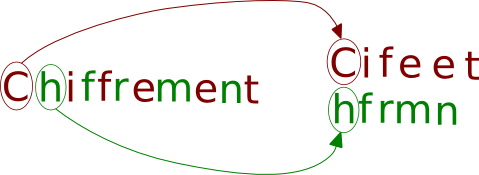
\includegraphics[scale=0.4]{images/Transposition.png}
  \end{center}
  \caption{le chiffre \emph{Rail Fence}, sur deux lignes.}
  \label{fig:Transposition}
\end{figure}

La plupart des chiffres de transposition utilisent des tableaux pour
chiffrer, il suffit alors d'écrire le message initial dans un tableau
d'une taille donnée, et de faire quelques opérations sur ce tableau
afin de «~mélanger~» les lettres. On peut facilement représenter cela
à l'aide des matrices : utilisons une matrice de 5
colonnes, dans laquelle nous écrivons «~chiffrement par transposition
». Un problème se pose alors pour la dernière ligne, elle n'est pas
complète ; deux choix s'offrent alors à nous : 
\begin{itemize}
  \item laisser ces cases vides~;
  \item utiliser des «~caractères nuls~», caractères aléatoires qui ne
    servent qu'à compléter la matrice et éventuellement à perturber la
    cryptanalyse du message chiffré.
\end{itemize}
Pour cet exemple, nous allons choisir la seconde méthode, et ajouter
les caractères G, O, K et Z à la fin de la matrice (figure
\ref{fig:TranspositionMatriceNul}).
\begin{figure}[h]
  \begin{center}
  $
  \left(
    \begin{array}{ccccc}
      C & H & I & F & F \\
      R & E & M & E & N \\
      T & P & A & R & T \\
      R & A & S & P & O \\
      S & I & T & I & O \\
      N & G & O & K & Z 
    \end{array}
  \right)
  $
  \end{center}
  \caption{le message écrit sous forme de matrice, avec l'ajout de
    caractères nuls.}
  \label{fig:TranspositionMatriceNul}
\end{figure}

Ensuite, nous allons changer l'ordre des colonnes en attribuant un
nombre à chacune des colonnes, et en les replaçant dans l'ordre des
nombres attribués. Le message chiffré se lira alors verticalement.
Nous pouvons éventuellement réitérer cette opération, c'est ce qu'on
appelle la \emph{double transposition} (ce qui rend la cryptanalyse plus
compliquée).

Les numéros attribués aux colonnes constitueront la clé ; pour
faciliter la mémorisation de celle-ci, nous pouvons utiliser un mot
où chaque lettre sera numérotée selon l'ordre alphabétique. Quand une
lettre apparaît plus d'une fois, la lettre la plus à gauche aura
l'indice le plus faible, la plus à droite l'indice le plus fort.

Utilisons ici la clé «~Pomme~», ce qui donne «~54231~» en chiffres,
nous réarrangeons donc les colonnes selon cet ordre (la dernière
colonne sera la première, la troisième la seconde, ...)

\begin{figure}[h]
  \begin{center}
  $
  \left(
    \begin{array}{ccccc}
      F & I & F & H & C \\ 
      N & M & E & E & R \\
      T & A & R & P & T \\
      O & S & O & A & R \\
      O & T & I & I & S \\
      Z & O & K & G & N
    \end{array}
  \right)
  $
  \end{center}
  \caption{la matrice réarrangée, selon la clé «~Pomme~».}
  \label{fig:TranspositionMatriceCode}
\end{figure}

Ainsi, le message codé sera «~FNTOOZIMASTOFEROIKHEPAIGCRTRSN~» et on
pourra facilement le déchiffrer en le réécrivant verticalement dans
une matrice possédant le même nombre de colonnes que la clé (5 ici),
en numérotant les colonnes de droite à gauche et en les remettant dans
l'ordre de la clé.

Nous avons utilisé ici un chiffre de transposition par colonnes, mais
il y a de nombreuses possibilités : par lignes, en diagonales, en
spirale, ...


\section{Chiffrement symétrique}
\subsection{Chiffrement par bloc}
\subsection{Chiffrement par flot}

\section{Chiffrement asymétrique}

\section{Les fonctions de hachages}
Les fonctions de hachages sont principalement utilisé en cryptographie
pour assurer l'intégrité des données. Une fonction de hachage produit
ce qu'on appelle communément un \emph{hash} ou \emph{somme de
  contrôle}  de taille fixe à partir de
données de taille indéfinie. Ceci peut amener à des \emph{collisions},
c'est à dire que deux données différentes peuvent donner la même somme
de contrôle, elles seront alors considérées comme identiques et cela
peut poser de sérieux problèmes de confidentialitée, de sécurité, ...

Dans ce chapitre, nous allons plus nous focaliser sur les méthodes
utilisées pour calculer la somme à partir des données, nous
regarderons en détail les problèmes de sécurités posés dans le
chapitre \ref{SecuriteHash}, page \pageref{SecuriteHash}.

%TODO

